%!TEX root=paper.tex
\section{Evaluation}\label{sec:evaluation}

We evaluate on the standard object detection benchmark: the PASCAL VOC \cite{pascal-voc-2010}.
In all cases, the CNN region classifiers are trained on the PASCAL VOC 2007 trainval set.
The parameters of our methods are set by training or cross-validation on the VOC 2007 val set.
We evaluate on the VOC 2007 test set.

The R-CNN software was used as available in June 2014\footnote{\url{https://github.com/rbgirshick/rcnn}}.
That software relies on Selective Search \cite{Uijlings-IJCV-2013} region proposals.
Different images are proposed different numbers of regions.
\autoref{fig:roi_hist} shows the distribution of number of regions on the validation set, with the parameters of the R-CNN.

An additional parameter is the size of each batch of regions that goes through the CNN.
We set batch size to 100 regions, and observe that it takes on average 500 ms to process them with the CNN.
In all experiments, we use Ubuntu 12.04, Intel i5 3.2GHz CPU, and NVIDIA Tesla K40 GPU.

The scoring function for the Region Statistics, Pixel Gradient, and Pyramid R-CNN features is trained by a logistic regression classifier onto the supervised signal of region overlap with ground truth on the validation dataset.
The classifier is optimized by stochastic gradient descent, and its regularization parameter is cross-validated.

The result plots and details are shown in \autoref{fig:voc2007_results} and \autoref{tab:results}.

\begin{figure}[ht]
\centering
\begin{subfigure}[b]{0.52\linewidth}
    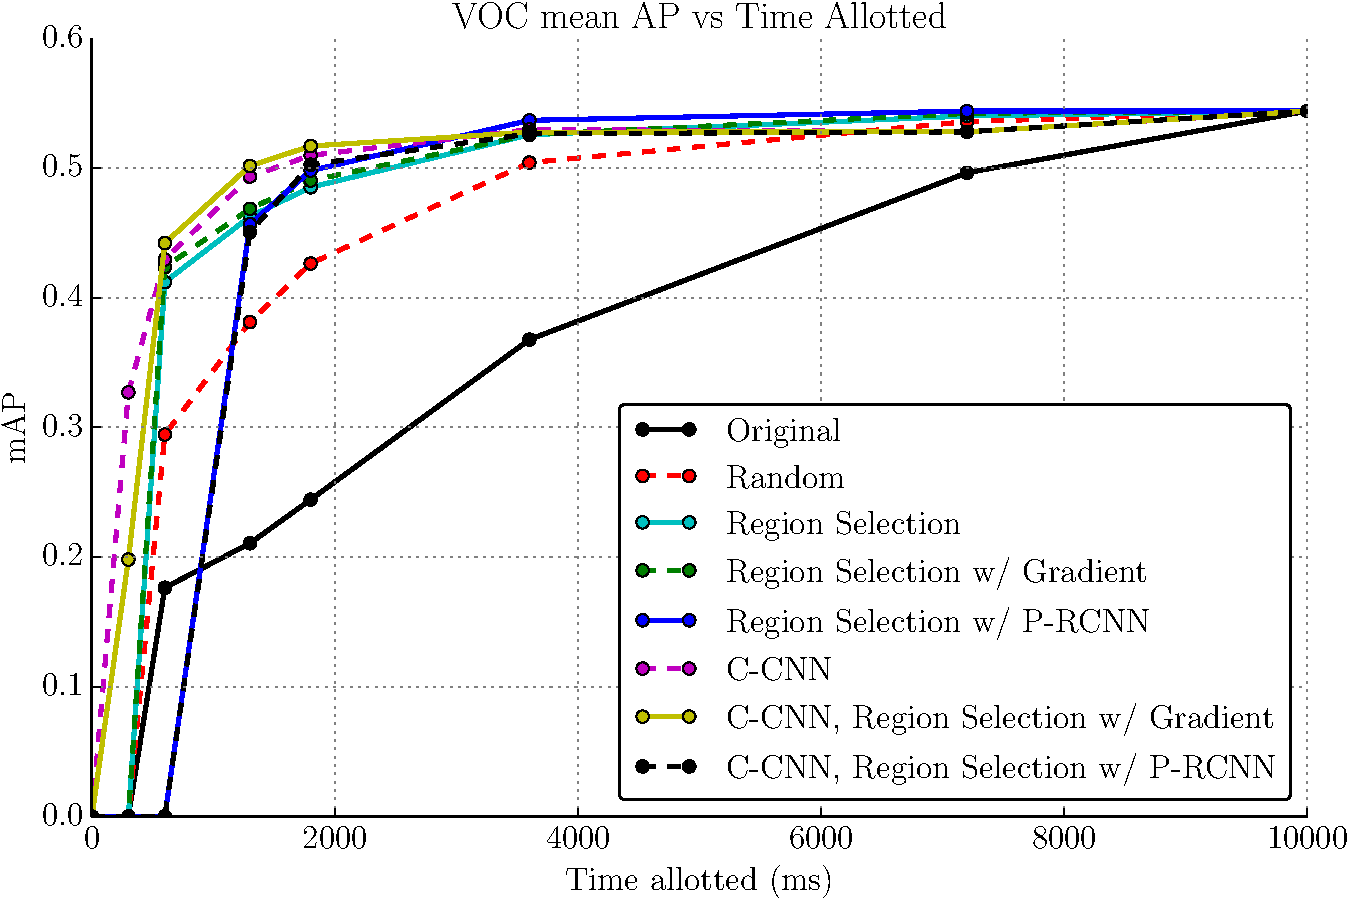
\includegraphics[width=\linewidth]{figures/_apvst_final.pdf}
    \caption{mAP vs. time allotted for detection}\label{fig:apvst}
\end{subfigure}\hfill
\begin{subfigure}[b]{0.45\linewidth}
    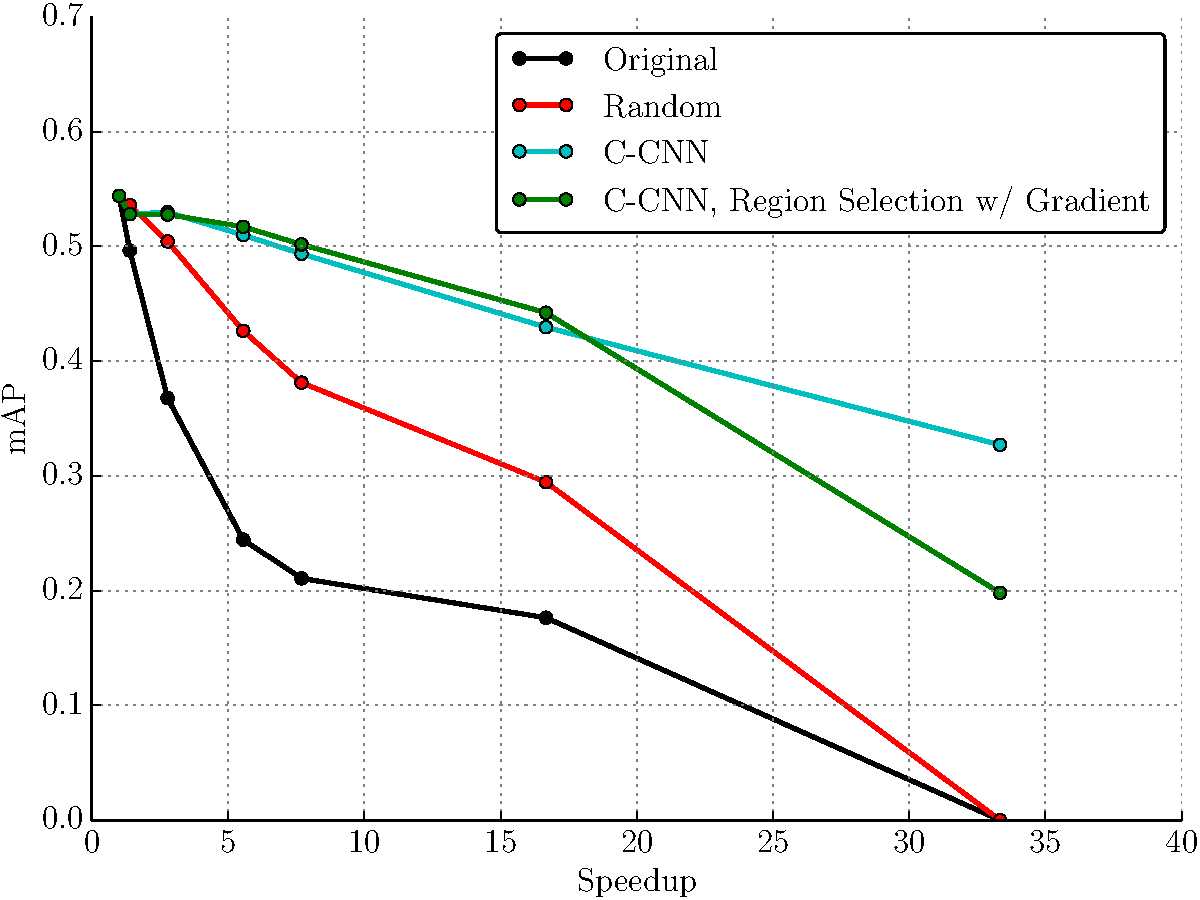
\includegraphics[width=\linewidth]{figures/_speedup_final_abs.pdf}
    \caption{mAP vs. speed-up factor}\label{fig:speedup}
\end{subfigure}
\caption{
Results on the PASCAL VOC 2007 dataset.
(a) On the left-hand mAP vs. Time plot, we can compare APs at a given allotted time point.
For example, at 1300 ms, random region selection gets about 0.42 mAP, while our best method (C-CNN with gradient-based region selection) obtains 0.50 mAP.
(b) On the right-hand speed-up plot, we can compare speed-ups at a given mAP point.
For example, we can see that we should obtain mAP of 0.40 at around 20x speedup with our method.
}\label{fig:voc2007_results}
\end{figure}

\begin{table}[ht]
\centering
\caption{
Full table of AP vs. Time results on PASCAL VOC 2007.
Best performance for each time point is in bold.
}\label{tab:results}
\small{
\begin{tabular}{lrrrrrrrr}
\toprule
Time allotted (ms)                  &  0     &  300   &  600   &  1300  &  1800  &  3600  &  7200  &  10000 \\
\midrule
Original                            &  0 &  0.000 &  0.176 &  0.211 &  0.244 &  0.368 &  0.496 &  0.544 \\
Random                              &  0 &  0.000 &  0.295 &  0.381 &  0.426 &  0.504 &  0.536 &  0.544 \\
Region Selection                    &  0 &  0.000 &  0.412 &  0.463 &  0.485 &  0.526 &  0.540 &  0.544 \\
Region Selection w/ Gradient        &  0 &  0.000 &  0.424 &  0.469 &  0.490 &  0.526 &  0.542 &  0.544 \\
Region Selection w/ P-RCNN          &  0 &  0.000 &  0.000 &  0.457 &  0.498 &  0.537 &  0.544 &  0.544 \\
C-CNN                               &  0 &  0.327 &  0.430 &  0.493 &  0.510 &  0.530 &  0.528 &  0.544 \\
C-CNN, Region Selection w/ Gradient &  0 &  0.198 &  0.442 &  0.502 &  0.517 &  0.528 &  0.528 &  0.544 \\
C-CNN, Region Selection w/ P-RCNN   &  0 &  0.000 &  0.000 &  0.451 &  0.503 &  0.527 &  0.528 &  0.544 \\
\bottomrule
\end{tabular}

}
\end{table}

\subsection{Experiments}
\begin{description}
  \item[Original] \hfill \\
  The original order of the Selective Search regions of interest.
  This order is influenced by the hierarchical segmentation of their method, and so has sequences of highly overlapping regions.
  \item[Random] \hfill \\
  A completely blind permutation of the original order.
  \item[Region Selection] \hfill \\
  The region statistics feature from \autoref{sec:region} is always used.
  Additionally, we consider either the Pixel Gradient and the Pyramid R-CNN features.
  These two features have a \emph{setup time}: the gradient forward-back propagation takes 20 ms, and the Pyramid R-CNN takes a whopping 800 ms.
  \item[Cascaded CNN]
  The Cascaded CNN model, as described in \autoref{sec:ccnn}.
  The first experiment (C-CNN) takes batches of regions in a random order.
  The next two experiments also make use of the Region Selection methodology, and the two fast features of Pixel Gradient and the Pyramid R-CNN.
\end{description}

\subsection{Analysis}
Since the time to process a full batch with a non-cascaded CNN is 500 ms, there are no results for non-cascaded baselines at 300 ms.
At this time, the Cascaded CNN without any region ordering is best.
A reason for why C-CNN with Region Selection is not as good at this point is that the region selection presents better region candidates, with fewer rejection opportunities, and thus has less coverage of the image.

At 600 ms, C-CNN method have had more than one batch go through, and the Region Selection is giving it a lead over the simple C-CNN.
Both method are better than the baseline non-cascaded methods for this entire duration.
This changes once the Pyramid R-CNN has time to compute and to run through a few batches.
The later times show best performance from the Region Selection with that feature.

\begin{figure}
\centering
\begin{subfigure}[b]{0.52\linewidth}
    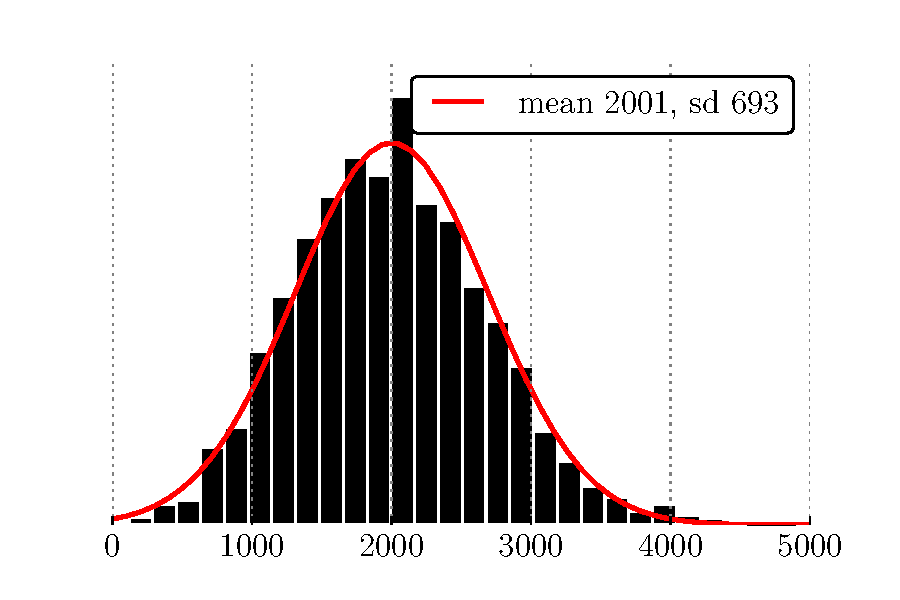
\includegraphics[width=\linewidth]{figures/roi_hist.pdf}
    \caption{Distribution of number of regions per image.}\label{fig:roi_hist}
\end{subfigure}\hfill
\begin{subfigure}[b]{0.33\linewidth}
    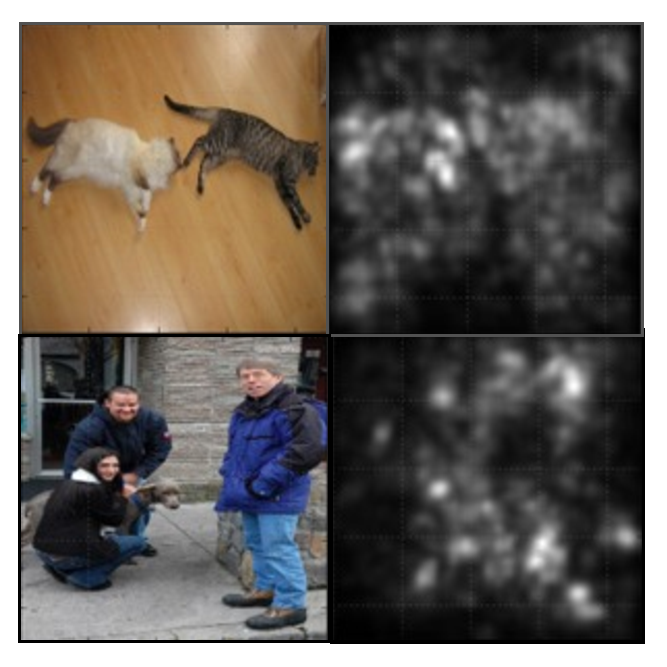
\includegraphics[width=\linewidth]{figures/gradient.pdf}
    \caption{Example of the CNN gradient.}\label{fig:gradient}
\end{subfigure}
\caption{}
\end{figure}
